\documentclass[11pt]{article}
\usepackage[utf8]{inputenc}
\usepackage[french]{babel}
\usepackage{graphicx}
\usepackage[T1]{fontenc}
\usepackage{lmodern}
\usepackage{amsmath}
\usepackage{amsfonts}
\usepackage{amssymb}
\usepackage{ifthen}
\usepackage{multicol}
\usepackage{fancyhdr}
\newcommand{\marge}{18mm}
\usepackage[left=\marge,right=\marge,top=\marge,bottom=\marge]{geometry}
\pagestyle{fancy}
\setlength{\headheight}{14pt}
\chead{\ifthenelse{\thepage=1}{
 \textbf{Nom :}
  \makebox[12em]{\dotfill}
  \hspace{2em}
  \textbf{Pr\'enom :}
  \makebox[12em]{\dotfill}}{}}
\rfoot{\ifthenelse{\thepage=1}{\textit{(tournez la page s.v.p)}}{}}
\renewcommand{\headrulewidth}{0pt}
\linespread{1.3}
\setlength{\columnseprule}{0.2pt}
 
% Commandes sp\'ecifiques pour les QCM
\newboolean{correction}
% true pour afficher la correction
% false pour la masquer
\setboolean{correction}{false}
\newcounter{QNumber}
\newcommand{\Question}[2][:]{
 \stepcounter{QNumber}
  \noindent\textbf{Question \theQNumber} --
  #2~#1}
\newenvironment{Reponse}{
 \begin{list}{$\square$}{\leftmargin=4em}}{
 \end{list}\vspace{1em}}
\newcommand{\Vrai}{
 \item[\ifthenelse{\boolean{correction}}{$\blacksquare$}{$\square$}]}
\newcommand{\Faux}{\item[$\square$]}
 
\def\N{\mathbb N}
\def\R{\mathbb R}
\def\Q{\mathbb Q}
\def\Z{\mathbb Z}
\begin{document}
  \begin{center}
    \bfseries\LARGE
    \textit{INFO I31, partiel 2013}\large
  \end{center}
  \sffamily
  \begin{itshape}
    Pour chaque question, r\'epondez directement sur la feuille.
Quand vous avez le choix, il n'y a qu'une seule bonne r\'eponse par question. Lisez et comprenez les questions avant d'y r\'epondre~! Tous les documents sont autorisés, mais pas la copie de votre voisin.
  \end{itshape}
  \begin{multicols}{2}
 
\Question{D\'eroulez l'algorithme d'Euclide pour calculer le PGCD de 187 et 55}

~\\
~\\
~\\
~\\
~\\

\Question{D\'eroulez l'algorithme d'Euclide \'etendu (ou Bezout) pour $a=187$ et $b=55$.
$u$ et $v$ sont tels que $au+bv=g=PGCD(a,b)$; $r=a \mod b$, et $q=\lfloor \frac{a}{b}\rfloor$
est le quotient de $a$ par $b$}
{\LARGE
$$
\begin{array}{|c|c|c|c||c|c|c|}
\hline
a & b & r & q & g & u & v \\
\hline
187 & 55 & \quad &  \quad &  \quad &  \quad& \\
    &     & & & & & \\
    &     & & & & & \\
    &     & & & & & \\
\hline
\end{array}$$
}


\Question{Citez les noms de 3 algorithmes de tri}
~\\
~\\

\Question{Citez les noms de 3 algorithmes calculant les plus courts chemins dans un graphe}
~\\
~\\




\Question{Donnez les formules n\'ecessaires pour le calcul r\'ecursif 
de $a^n$ ($a$ est une matrice carrée, à valeurs enti\`eres). N'oubliez pas le ou les cas terminaux}  


~\\
~\\
~\\
~\\
~\\

\begin{center}
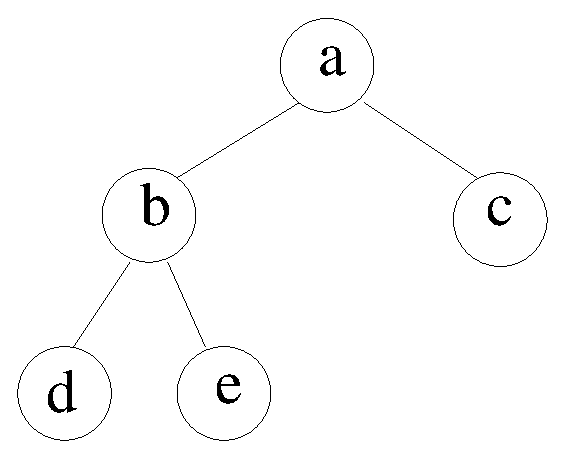
\includegraphics[width=0.7\linewidth]{arbrebin.eps}
\end{center}
\Question{Dans l'arbre ci-dessus, l'affichage: a, b, c, d, e est obtenu par}
\begin{Reponse}
\Vrai un parcours en largeur
\Faux un parcours en  profondeur
\end{Reponse}


\Question{Dans l'arbre ci-dessus, l'affichage: a, b, d, e, c est obtenu par}
\begin{Reponse}
\Faux un parcours en largeur
\Vrai un parcours en  profondeur
\end{Reponse}


\Question{Un algorithme optimal de tri,  n'utilisant que des comparaisons entre 2 \'el\'ements,
n\'ecessite}
 \begin{Reponse}
\Vrai $O(n \log n)$ comparaisons pour trier $n$ \'el\'ements
\Faux $O(n^2)$ comparaisons 
\Faux $O(n)$ comparaisons
\Faux un nombre exponentiel de comparaisons
\end{Reponse}


\Question{L'arbre binaire de hauteur 0 contient 0 éléments.
Celui de hauteur 1 contient 1 élément.
Combien d'éléments contient l'arbre complet de hauteur $h$ }
~\\
~\\
~\\
\Question{L'arbre binaire de hauteur 0 contient 0 éléments, et donc 0 feuilles.
Celui de hauteur 1  contient 1 élément, qui est une feuille.
Combien  de feuilles (éléments les plus profonds dans l'arbre) contient
l'arbre complet de hauteur $h$ } 
~\\
~\\
~\\


\begin{center}
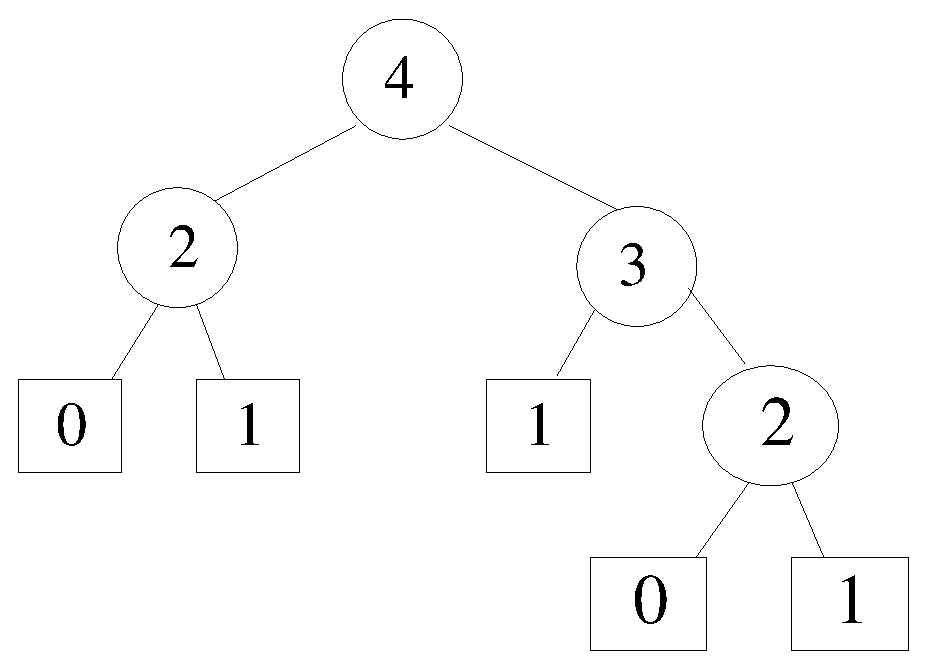
\includegraphics[width=0.7\linewidth]{arbreFibonacci.eps}
\end{center}

\Question{L'arbre de Fibonacci $T_4$ est dessin\'e ci-dessus. $T_0$ est une feuille portant l'\'etiquette 0,
$T_1$ est une feuille portant  l'\'etiquette 1; pour $n>1$, $T_n$ est un noeud binaire, dont le fils gauche est $T_{n-2}$ et dont le fils droit est $T_{n-1}$. Donnez une formule r\'ecursive pour 
le nombre d'\'el\'ements (feuilles ou sommets), not\'e $|T_n|$,  de $T_n$, pour $n>1$}

~\\
~\\



\Question{D\'efinissez $U_n$ le nombre de feuilles \'etiquet\'ees 1 de $T_n$. Que constatez-vous}

~\\
~\\
~\\

\Question{D\'efinissez $Z_n$ le nombre de feuilles \'etiquet\'ees 0 de $T_n$}

~\\
~\\
~\\

\Question{Remplissez le tableau suivant, o\`u $U_n$ est le nombre de feuilles \'etiquet\'ees 1 de $T_n$,
$Z_n$ le nombre de feuilles \'etiquet\'ees 0 de $T_n$}

{\Large
$$
\begin{array}{|c|c|c|c|c|c|c|c|c|c|c|}
\hline
n & 0 & 1 & 2 & 3 & 4 & 5 & 6 & 7 & 8 & 9 \\
\hline
|T_n| & & & & & & & & & &  \\
\hline
U_n & & & & & & & & & &  \\
\hline
Z_n & & & & & & & & & &  \\
\hline
\end{array}
$$
}

\end{multicols}
\end{document}
\Question{Prolongez de fa\c{c}on logique la suite de Fibonacci aux nombres n\'egatifs}
$$\begin{array}{|c|cccccccccccc|}
\hline
i & -6 & -5 & -4 & -3 & -2 & -1 & 0 & 1 & 2 & 3 & 4 & 5  \\
\hline
F_i & & & & & & & 0 & 1 & 1 & 2 & 3 & 5  \\
\hline
\end{array}
$$


\Question{Vous constatez que, pour $n\in \N$,  $F_{-2n}$ est \'egal \`a}

~\\

\Question{Vous constatez que, pour $n\in \N$,  $F_{-2n-1}$ est \'egal \`a}

~\\
 

\Question{ Soient $\phi=\frac{1}{2}(1+\sqrt{5})\approx 1.618$ et $\phi'=\frac{1}{2}(1-\sqrt{5})\approx -0.618$~; ce sont les deux racines de $x^2-x-1=0$. 
D\'efinissons $f(n)=\frac{1}{\sqrt{5}}(\phi^n - \phi'^n)$.
Donnez la valeur de $f(0), f(1), f(2), f(3)$} 

\Question{Par r\'ecurrence, prouvez que $F_n=f(n)$}

~\\
~\\
~\\
~\\
~\\

\Question{Le temps d'ex\'ecution d'un algorithme  est
$T(n)$ pour une donn\'ee de taille $n$, o\`u $T(1)=1$ et $T(n)=3 T(n/2)+n$.
Prouver par r\'ecurrence que $T(2^k) = 3^{k+1}-2^{k+1}$}

~\\
~\\
~\\
~\\
~\\

\Question{Prouvez que $3^{\log_2 n}$ est en $O(n ^{log_3 2})$ (Remarque: $\log_3 2\approx 1.5849625$)}

~\\
~\\
~\\
~\\
~\\


\Question{Calculer le produit scalaire entre 2 vecteurs de $n$ nombres flottants $u=(u_i)$ et $v=(v_i)$ n\'ecessite}
\begin{Reponse}
\Faux $O(\log n)$ op\'erations flottantes
\Vrai $O( n)$ op\'erations flottantes
\Faux $O( n\log n)$ op\'erations flottantes
\Faux $O( n^2)$ op\'erations flottantes
\end{Reponse}

\Question{Calculer le produit entre une matrice carr\'ee quelconque de taille $n\times n$, contenant $n^2$  nombres flottants, et un vecteur colonne de $n$ \'el\'ements ($n$ nombres flottants)
n\'ecessite}
\begin{Reponse}
\Faux $O(n \log n)$ op\'erations flottantes
\Faux  $O(n )$ op\'erations flottantes
\Vrai  $O(n^2 )$ op\'erations flottantes
\Faux ce n'est pas toujours possible
\end{Reponse}

\Question{Calculer le produit entre deux matrices carr\'ees de taille  $n\times n$, en appliquant la formule~: $C_{lc}=\sum_{k=1}^n A_{lk}\times B_{kc}$, n\'ecessite}
\begin{Reponse}
\Faux $O(n \log n)$ op\'erations flottantes
\Faux  $O(n )$ op\'erations flottantes
\Vrai  $O(n^2 )$ op\'erations flottantes
\Vrai  $O(n^3 )$ op\'erations flottantes
\Faux ce n'est pas toujours possible (la matrice doit \^etre inversible, par exemple).
\end{Reponse}

\Question{La m\'ethode de puissance rapide pour calculer $M^k$ ($M$ est une matrice carr\'ee de taille $n\times n$, et $k$ est un entier naturel)  n\'ecessite}  
\begin{Reponse}
\Faux in\'evitablement $k-1$ (donc $O(k)$) multiplications de matrices carr\'ees de taille $n\times n$
\Vrai $O(\log k)$ multiplications de matrices carr\'ees de taille $n\times n$
\Vrai $O(k\log k)$ multiplications de matrices carr\'ees de taille $n\times n$
\Faux ce n'est pas toujours possible (la matrice doit \^etre inversible, par exemple).
\end{Reponse}


\Question{Trouver l'\'el\'ement le plus petit dans une liste non ordonn\'ee de taille $n>0$  n\'ecessite}
\begin{Reponse} 
\Faux $O(1)$ comparaisons
\Faux $O(n^2)$ comparaisons
\Vrai $O(n)$ comparaisons
\Faux $O(\log n)$ comparaisons
\end{Reponse} 

\Question{Trouver l'\'el\'ement le plus petit dans une liste tri\'ee par ordre croissant et de taille $n>0$  n\'ecessite}
\begin{Reponse} 
\Vrai $O(1)$ comparaisons
\Faux $O(n^2)$ comparaisons
\Vrai $O(n)$ comparaisons
\Faux $O(\log n)$ comparaisons
\end{Reponse}


\Question{
Un \'etudiant programme le tri rapide ("quicksort") d'une liste $L$ ainsi~: si $L$  contient moins de 2 \'el\'ements, alors elle est d\'ej\`a tri\'ee. Sinon, l'\'etudiant choisit un \'el\'ement $p$  dans $L$. Il partitionne $L$  
en 3 sous listes, la liste $L_1$ des \'el\'ements dans $L$ inf\'erieurs \`a $p$, la liste $L_2$ des \'el\'ements dans $L$
\'egaux \`a $p$,  
la liste $L_3$  des \'el\'ements dans $L$ sup\'erieurs \`a $p$. Il trie r\'ecursivement les 3 listes, puis concat\`ene les r\'esultats. 
Qu'en pensez-vous}
\begin{Reponse}
\Faux la m\'ethode est correcte mais la complexit\'e est modifi\'ee
\Faux la m\'ethode est correcte et la complexit\'e est inchang\'ee
\Vrai la m\'ethode est incorrecte ; elle boucle quand  $L$ contient deux (ou davantage) \'el\'ements \'egaux \`a $p$.
\Faux la m\'ethode est incorrecte car $L_2$ n'est jamais vide, puisqu'elle contient $p$.
\end{Reponse}


\Question{Pour le calcul de l'arbre couvrant minimum d'un graphe connexe, 
un \'etudiant propose l'algorithme suivant: si le graphe est un arbre, alors ins\'erer cet arbre dans l'arbre couvrant minimum;
sinon d\'ecomposer le graphe $G$ en 2 graphes de taille \`a peu pr\`es moiti\'e, $G_1$, et $G_2$, tous deux connexes; calculer
l'arbre couvrant minimum de $G_1$; calculer l'arbre couvrant minimum de $G_2$; joindre ces deux arbres par l'ar\^ete de co\^ut
 minimum entre $G_1$ et $G_2$ (cette ar\^ete a un sommet dans $G_1$ et un sommet dans $G_2$). 
Que pensez-vous de cet algorithme} 

\begin{Reponse}
\Faux il est correct
\Faux il est difficile de partitionner un graphe connexe en deux sous graphes connexes ayant (\`a peu pr\`es) deux fois moins de sommets; c'est pourquoi cet algorithme n'est pas utilis\'e
\Vrai il est incorrect, et voici un contre exemple simple (au plus 4 sommets!) :

~ \\
 ~ \\
~ \\
~ \\

\end{Reponse}


\Question{Une matrice de Vandermonde a la structure suivante~:
$$M= \left( \begin{array}{ccccc}
1 & 1 & 1 & \ldots & 1 \\
1 & w & w^2 & \ldots & w^{n-1} \\
1 & w^2 & w^4 & \ldots &  w^{2(n-1)} \\
\ldots & \ldots & \ldots & \ldots \\
1 & w^{n-1} &  w^{2n-2} &  \ldots & w^{(n-1)^2} \\
\end{array} \right)
$$ o\`u $n$ est une puissance de 2.
Si de plus $w$ est une racine $n$ i\`eme de l'unit\'e, alors le produit avec un vecteur colonne quelconque de taille $n$}
\begin{Reponse}
\Vrai peut se faire en $O(n \log n)$ (avec l'algorithme de la transform\'ee rapide de Fourier) 
\Vrai ne  peut pas se faire en moins que  $O(n)$
\Faux ne peut pas se faire en moins que $O(n^2)$
\end{Reponse}

\Question{Pour $n=8$ (donc $w^8=1$), \'ecrire la ligne de la matrice de Vandermonde commen\c{c}ant par $1$ puis  $w^3$, en simplifiant
(c'est \`a dire en \'eliminant les puissances plus grandes que 7)}

~\\
~\\
~\\
~\\

\Question{Idem, pour $n=8$, \'ecrire la ligne de la matrice de Vandermonde commen\c{c}ant par $1$ puis  $w^6$}

~\\
~\\
~\\
~\\

\Question{Dans le probl\`eme de la somme, un ensemble $E$ de $n$ entiers positifs $e_1 \ge e_2 \ge \ldots \ge e_n$ est donn\'e, ainsi
qu'un entier $0<S < \sum_1^n e_i$. Il faut trouver le sous ensemble $X$ de $E$ dont la somme des \'el\'ements
est maximum, mais inf\'erieure ou \'egale \`a $S$.  Pour tout ensemble $K$, on note $\sigma(K)$ la somme des \'el\'ements de $K$.
L'algorithme glouton calcule $X_0=\emptyset$ (donc $s(X_0)=0$);  puis, 
pour $i$ de 1 \`a $n$, il calcule $X_i= X_{i-1} \cup \{e_i\}$ si $e_i + \sigma(X_{i-1}) \le S$, et
$X_i= X_{i-1}$ sinon. Avec $E=100,25,20,10,1,1,1$ et $S=40$, donnez les valeurs de $X_0, X_1, \ldots X_7$, et les $\sigma(X_i)$ correspondants}

~\\
~\\
~\\
~\\
~\\
~\\
~\\

\Question{
Cet algorithme donne-t-il un sous ensemble $X_n$}
\begin{Reponse} 
\Vrai toujours correct ($s(X_n)\le S$), mais pas forc\'ement optimal : donnez un exemple simple ($n<5$) o\`u $X_n$ n'est pas optimal\\
~
\Faux toujours correct, et toujours optimal
\Faux pas toujours correct, mais optimal :  donnez un exemple simple ($n<5$) \\
~ 
\Faux souvent correct, et souvent optimal
\Faux ni correct ni optimal : donnez un exemple simple ($n<5$) \\
~
\Faux toutes les r\'eponses pr\'ec\'edentes sont fausses 
\end{Reponse}


\Question{Arthur conjecture que si, dans un graphe non orient\'e, tous les sommets distincts soit sont voisins, 
soit ont un voisin en commun, alors il existe au moins un sommet qui est voisin de tous les autres.  Que pensez vous de cette conjecture}
\begin{Reponse}
\Faux elle est vraie
\Vrai elle est fausse et vous en dessinez un contre exemple simple \\
~\\
\end{Reponse}


\end{multicols}
\end{document}
